\documentclass{article}
\usepackage{amsmath}
\usepackage{amssymb}
\usepackage{float}
\usepackage{ifthen}
\usepackage{tikz}
\newcommand{\pred}{\mathcal{O}}
\newcommand{\conject}{\mathcal{C}}
\newcommand{\modrow}{\mathcal{R}}
\newcommand{\minipascal}{\mathcal{P}}

\newcommand{\drawemptyrow}[4]{
    \node at (#2/4, #3/4) {#4};
    \node at (#2/-4, #3/4) {#4};
  }

\newcommand{\drawrow}[4]{
  \drawemptyrow{#1}{#2}{#3}{#4}
  \foreach \i in {0,...,#1}{
    \node at (#2/-4-\i/-2,#3/4){#4};
    %\drawemptyrow{\i}{#2+\i}{#3}
  }
}

\newcommand{\drawoddtriangle}[2]{
  \foreach \i in {0,...,7}{
    \drawemptyrow{\i}{#1+0+\i}{#2+7-\i}{1}
   }
   \drawrow{7}{#1+7}{#2+21}{1}
  }
\begin{document}

\begin{center}\item \section*{Problem}\end{center}

Find all $n \geq 0$ such that ${n \choose k}$ is odd, for all $0\leq k \leq n$.

\begin{center}\item \section*{Solution}\end{center}

Let $\pred(n) = $``${n \choose k}$ is odd, for all $0 \leq k \leq n$.''

First, note the first few values for $n$ which satisfy $P$.
\begin{align*}
  0 &\mapsto (1)\\
  1 &\mapsto (1,1)\\
  3 &\mapsto (1,3,3,1)\\
  7 &\mapsto (1,7,21,35,35,21,7,1)\\
  15 &\mapsto (1,15,105,455,1365,3003,5005,6235,6435,5005,3003,1365,455,105,15,1)
\end{align*}


Note that they increase by powers of 2. In fact, each of the $n$ we observed are 1 less than a power of 2. Thus, we shall conjecture that $\pred(n)$ is true iff $n = 2^x-1$, for some $x \geq 0$.

Let $\conject(n)$ = ``$\pred(n)$ is true iff $n$ = $2^x-1$, for some $x\geq 0$.


\begin{center}\item \subsubsection*{Proof of $\conject$ by Induction on n}\end{center}

First, define $\modrow(n,i,j) = $ the sequence of elements in row $n$ of Pascal's Triangle mod 2 from index $i$ to $j$. If $i$ and $j$ are omitted, it is to be assumed $\modrow(n) = \modrow(n, 0, n)$.

As an example, $\modrow(1) = \{1,1\}$, $\modrow(2)= \{1,0,1\}$.
\begin{center}\item \textbf{Base Cases} \end{center}

When $n = 0 = 2^0-1$ or $n=1=2^1-1$, $\pred(n)$ is true.

\begin{center}\item\textbf{Inductive Case} \end{center}

Let $n\geq 1$ and assume $\conject(n)$ is true. Without loss of generality, assume $\pred(n)$ is true. This implies the following:
\begin{enumerate}
  \item $n = 2^x - 1$, for some $x \geq 0$.
  \item $\modrow(n) = \{\underbrace{1,1,...1,1}_{n+1}\}$.
\end{enumerate}

\begin{figure}[H]
\centering
\begin{tikzpicture}
  \drawoddtriangle{0}{0}
\end{tikzpicture}
\caption {Pascal's Triangle mod 2 up to row $n$. The internal values are not significant for our proof.}.
\end{figure}

We want to show that $\pred(x)$ is false for $n < m < 2^{x+1}-1 = 2n+1$, and $\pred(m)$ is true when $m = 2n+1$.

By Pascal's Relation, if $\modrow(n) = \{1,\underbrace{1,...,1}_{n-1},1\}$, 
then $\modrow(n+1) = \{1,\underbrace{0,0,...0,0}_{n},1\}$.

\begin{figure}[H]
\centering
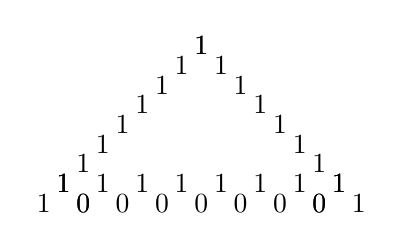
\begin{tikzpicture}
  \drawoddtriangle{0}{0}
  \drawemptyrow{8}{8}{20}{1}
  \drawrow{6}{6}{20}{0}
\end{tikzpicture}
\end{figure}

Similarly, by repeatedly applying Pascal's Relation, we can derive that:
$$
\forall 0 \leq r \leq n-1, \forall 1+r\leq c \leq n+1+r-1+r=n, {n+1+r \choose c} \equiv_2 0
$$
In other words, the cluster of even integers in row $n+1$ will `fold' in, in particular in the shape of a downward triangle. Consequently, $\pred(x)$ is false for $n+1\leq x \leq n+1+n-1 = 2n$.

\begin{figure}[H]
\centering
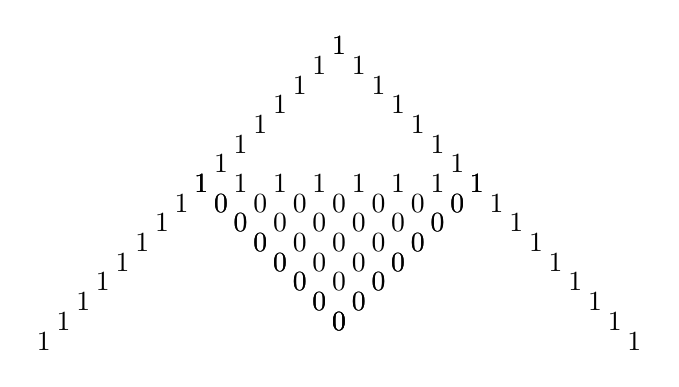
\begin{tikzpicture}
  \drawoddtriangle{0}{0}
  \drawemptyrow{8}{8}{20}{1}
  \drawrow{6}{6}{20}{0}
  \drawemptyrow{9}{9}{19}{1}
  \drawrow{5}{5}{19}{0}
  \drawemptyrow{10}{10}{18}{1}
  \drawrow{4}{4}{18}{0}
  \drawemptyrow{11}{11}{17}{1}
  \drawrow{3}{3}{17}{0}
  \drawemptyrow{12}{12}{16}{1}
  \drawrow{2}{2}{16}{0}
  \drawemptyrow{13}{13}{15}{1}
  \drawrow{1}{1}{15}{0}
  \drawemptyrow{14}{14}{14}{1}
  \drawrow{0}{0}{14}{0}
  \drawemptyrow{15}{15}{13}{1}
\end{tikzpicture}
\end{figure}

Note that by Pascal's Relation, since
 ${n+1 \choose 1} \equiv_2 0$ and ${n+1 \choose 0} \equiv_2 1$,
 ${n+2 \choose 1} \equiv_2 1$. We can then recursively reapply this to get:
$$
\forall 0\leq r \leq n-1, {n+2+r \choose 1+r} \equiv_2 1
$$
By the symmetry of Pascal's Triangle, the reflection of this holds for the other side as well.

\begin{figure}[H]
\centering
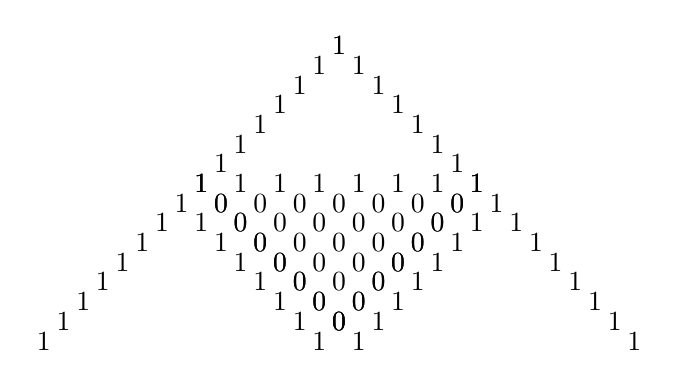
\begin{tikzpicture}
  \drawoddtriangle{0}{0}
  \drawemptyrow{8}{8}{20}{1}
  

  \drawrow{6}{6}{20}{0}
  \drawemptyrow{9}{9}{19}{1}
  \drawemptyrow{7}{7}{19}{1}

  \drawrow{5}{5}{19}{0}
  \drawemptyrow{10}{10}{18}{1}
  \drawemptyrow{8}{6}{18}{1}

  \drawrow{4}{4}{18}{0}
  \drawemptyrow{11}{11}{17}{1}
  \drawemptyrow{9}{5}{17}{1}

  \drawrow{3}{3}{17}{0}
  \drawemptyrow{12}{12}{16}{1}
  \drawemptyrow{7}{4}{16}{1}

  \drawrow{2}{2}{16}{0}
  \drawemptyrow{13}{13}{15}{1}
  \drawemptyrow{6}{3}{15}{1}

  \drawrow{1}{1}{15}{0}
  \drawemptyrow{14}{14}{14}{1}
  \drawemptyrow{5}{2}{14}{1}

  \drawrow{0}{0}{14}{0}
  \drawemptyrow{15}{15}{13}{1}
  \drawemptyrow{4}{1}{13}{1}
\end{tikzpicture}
\end{figure}

Since $\modrow(n+2,0,1) = \modrow(1,0,1)$, by Pascal's Relation we know that $\modrow(n+3,0,2) = \modrow(2,0,2)$. By recursively applying this, we get that:
$$
\forall 0 \leq i \leq n-1, \modrow(n+2+i,0,1+i) = \modrow(1+i,0,1+i)
$$

In other words, each row of this 'mini' pascal triangle mod 2 from rows $n+1$ to $n+1+n = 2n+1$ is identical to rows 0 to $n$ (by the symmetry of Pascal's Triangle, the reflection of this holds true as well).

Therefore, $\modrow(n+2+n-1=2n+1, 0, n) = \{\underbrace{1,1...,1,1}_{n+1}\}$ and
           $\modrow(2n+1,n+1, 2n+1) = \{\underbrace{1,1...1,1}_{n+1}\}$.

Combining these, we get that $\modrow(2n+1) = \{\underbrace{1,1..1,1}_{2n+2}\} \Rightarrow \pred(2n+1)$ is true.

\begin{figure}[H]
\centering
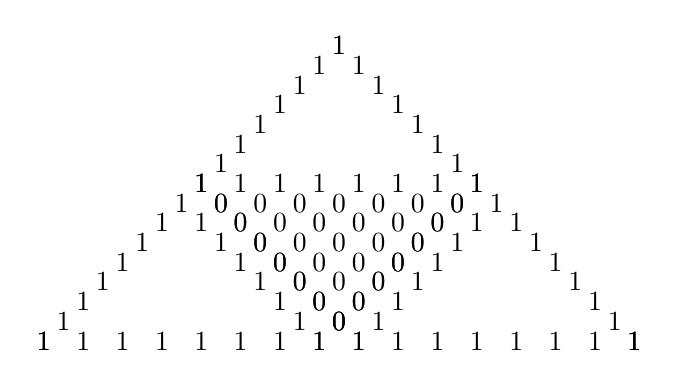
\begin{tikzpicture}
  \drawoddtriangle{0}{0}
  \drawemptyrow{8}{8}{20}{1}
  

  \drawrow{6}{6}{20}{0}
  \drawemptyrow{9}{9}{19}{1}
  \drawemptyrow{7}{7}{19}{1}

  \drawrow{5}{5}{19}{0}
  \drawemptyrow{10}{10}{18}{1}
  \drawemptyrow{8}{6}{18}{1}

  \drawrow{4}{4}{18}{0}
  \drawemptyrow{11}{11}{17}{1}
  \drawemptyrow{9}{5}{17}{1}

  \drawrow{3}{3}{17}{0}
  \drawemptyrow{12}{12}{16}{1}
  \drawemptyrow{7}{4}{16}{1}

  \drawrow{2}{2}{16}{0}
  \drawemptyrow{13}{13}{15}{1}
  \drawemptyrow{6}{3}{15}{1}

  \drawrow{1}{1}{15}{0}
  \drawemptyrow{14}{14}{14}{1}
  \drawemptyrow{5}{2}{14}{1}

  \drawrow{0}{0}{14}{0}
  \drawemptyrow{15}{15}{13}{1}
  \drawemptyrow{4}{1}{13}{1}

  \drawrow{15}{15}{13}{1}
\end{tikzpicture}
\end{figure}

Thus, $\conject(2n+1)$ is true, which means by mathematical induction, $\conject$ is true for all $n$.

\end{document}
